\chapter{Cenários de Teste}\label{cenariosTeste}
	Os cenários de teste tem como função apoiar no processo de observação sistemática, para que através deles a maquina de raciocínio seja avaliada e tal pergunta seja respondida: a máquina de racicínio está satisfatória?
	
	Os cenários de teste consistem em 9 conjuntos de missões distintas, criados no componente \textit{conjuntoMissoes.pl}, a fim de testar a saída do robô. Foram analisados os retornos do \textit{algoritmoDeDecisao}, que são as missões que devem ser efetuadas, e da \textit{stringDePontos}, que contém os pontos de cada missão escolhida.

	O gabarito para cada cenário de teste foi criado da seguinte forma: para o \textit{algoritmoDeDecisao}, foi feita uma análise manual da programação dinâmica, obtendo assim um resultado; e para a \textit{stringDePontos,} foram verificados se todos os pontos iniciais das missões eram x=0 e y=0, e os pontos finais condiziam com os especificados no arquivo \textit{pontoFinalMissao.pl}.

	As Tabelas de \ref{cenario01} a \ref{cenario09} mostram os cenários de teste, especificando a pontuação e o  tempo de cada um.

\begin{table}[!h]
\centering
\caption{Cenário de Teste 1}
\label{cenario01}
\begin{tabular}{lll}
Missão             & Pontuação & Tempo \\
Caminhão           & 20        & 28    \\
Sinal de Evacuação & 30        & 22    \\
Avião              & 30        & 13    \\
Galho              & 30        & 15    \\
Tsunami            & 30        & 15    \\
Ambulância         & 25        & 30    \\
Realocação         & 20        & 37    \\
Base de Isolamento & 30        & 26    \\
Obstáculos         & 31        & 40    \\
Elevar a Casa      & 25        & 15    \\
Família            & 33        & 26    \\
Segurança          & 36        & 26   \\
\end{tabular}
\end{table}


\begin{table}[!h]
\centering
\caption{Cenário de Teste 2}
\label{cenario2}
\begin{tabular}{lll}
Missão             & Pontuação & Tempo \\
Caminhão           & 20        & 28    \\
Sinal de Evacuação & 30        & 22    \\
Avião              & 30        & 13    \\
Galho              & 30        & 15    \\
Tsunami            & 30        & 15    \\
Ambulância         & 25        & 30    \\
Realocação         & 20        & 37 
\end{tabular}
\end{table}	

\begin{table}[!h]
\centering
\caption{Cenário de Teste 3}
\label{cenario3}
\begin{tabular}{lll}
Missão             & Pontuação & Tempo \\
Realocação         & 20        & 37    \\
Base de Isolamento & 30        & 26    \\
Obstáculos         & 31        & 40    \\
Elevar a Casa      & 25        & 15    \\
Família            & 33        & 26    \\
Segurança          & 36        & 26   
\end{tabular}
\end{table}

\begin{table}[!h]
\centering
\caption{Cenário de Teste 4}
\label{cenario4}
\begin{tabular}{lll}
Missão             & Pontuação & Tempo \\
Avião              & 30        & 13    \\
Galho              & 30        & 15    \\
Tsunami            & 30        & 15    \\
Ambulância         & 25        & 30    \\
Realocação         & 20        & 37    \\
Base de Isolamento & 30        & 26    \\
Família            & 33        & 26   
\end{tabular}
\end{table}

\begin{table}[!h]
\centering
\caption{Cenário de Teste 5}
\label{cenario5}
\begin{tabular}{lll}
Missão             & Pontuação & Tempo \\
Avião              & 30        & 13    \\
Tsunami            & 30        & 15    \\
Realocação         & 20        & 37    \\
Base de Isolamento & 30        & 26    \\
Obstáculos         & 31        & 40    \\
Elevar a Casa      & 25        & 15    \\
Família            & 33        & 26    \\
Segurança          & 36        & 26   
\end{tabular}
\end{table}

\begin{table}[!h]
\centering
\caption{Cenário de Teste 6}
\label{cenario6}
\begin{tabular}{lll}
Missão             & Pontuação & Tempo \\
Caminhão           & 20        & 28    \\
Sinal de Evacuação & 30        & 22    \\
Avião              & 30        & 13    \\
Galho              & 30        & 15    \\
Obstáculos         & 31        & 40    \\
Elevar a Casa      & 25        & 15    \\
Família            & 33        & 26    \\
Segurança          & 36        & 26   
\end{tabular}
\end{table}

\begin{table}[!h]
\centering
\caption{Cenário de Teste 7}
\label{cenario7}
\begin{tabular}{lll}
Missão             & Pontuação & Tempo \\
Tsunami            & 30        & 15    \\
Ambulância         & 25        & 30    \\
Realocação         & 20        & 37    \\
Base de Isolamento & 30        & 26    \\
Família            & 33        & 26    \\
Segurança          & 36        & 26   
\end{tabular}
\end{table}

\begin{table}[!h]
\centering
\caption{Cenário de Teste 8}
\label{cenario8}
\begin{tabular}{lll}
Missão             & Pontuação & Tempo \\
Sinal de Evacuação & 30        & 22    \\
Tsunami            & 30        & 15    \\
Ambulância         & 25        & 30    \\
Realocação         & 20        & 37    \\
Família            & 33        & 26    \\
Segurança          & 36        & 26   
\end{tabular}
\end{table}

\begin{table}[!h]
\centering
\caption{Cenário de Teste 9}
\label{cenario09}
\begin{tabular}{lll}
Missão             & Pontuação & Tempo \\
Sinal de Evacuação & 30        & 22    \\
Avião              & 30        & 13    \\
Galho              & 30        & 15    \\
Tsunami            & 30        & 15    \\
Ambulância         & 25        & 30    \\
Realocação         & 20        & 37    \\
Base de Isolamento & 30        & 26    \\
Obstáculos         & 31        & 40    \\
Elevar a Casa      & 25        & 15    \\
Família            & 33        & 26    \\
Segurança          & 36        & 26   
\end{tabular}
\end{table}
\clearpage

	Ao iniciar o primeiro cenário de teste, foram verificados os retornos acima especificados, sendo que todos estavam de acordo com o gabarito. Porém, o robô não executou o trajeto. Depois de avaliar o código do Traveller, foi percebido que a conexão \textit{bluetooth} estava sendo feita apenas em uma direção, que seria do computador para o NXT, tanto que era possível passar o código para o mesmo via \textit{bluetooth}. Entretanto, o NXT não estava conectando ao computador como deveria, e por esse motivo, aparecia a seguinte mensagem no visor: \textit{"No known devices"}.

	O Traveller, para passar o caminho ao NXT, tentava criar uma conexão \textit{bluetooth} utilizando o método \textit{getKnownDevice}, que procura na lista de devices do NXT o nome do computador, e realiza a conexão. Como a lista do NXT estava vazia, a conexão não era efetuada.

	A primeira tentativa para contornar o problema foi a utilização do método \textit{inquire}, que pesquisa a lista de dispositivos encontrados, pelo \textit{search} do robô, e com base nessa lista, ele adiciona o computador à lista de dispositivos conhecidos do NXT, utilizando o método \textit{addDevice}. Entretanto, nessa abordagem, o retorno do \textit{inquire} sempre vinha nulo, mesmo o NXT achando o computador quando realizada a busca manualmente.

	Analisando melhor a comunicação entre os módulos do Traveller, foi averiguado que o \textit{server} ficava sempre à espera da conexão que vinha do módulo \textit{robot}. Essa dinâmica foi invertida, pois como quem inicializa o Traveller é o Prolego, logo não existe a necessidade dessa espera. 

	Para fazer o \textit{robot} aguardar a conexão vinda do \textit{server}, foi utilizado o método \textit{waitForConnection}. Com o robô em espera da conexão, o \textit{server} abre uma conexão com ele através do método \textit{NXTInfo}, que recebe como argumentos o nome do robô, no caso GTX, e o endereço MAC dele.

	Ao realizar essas modificações, a conexão foi efetuada com sucesso e o robô começou a executar os caminho dos pontos passados. No entanto, foi averiguado um problema de odometria ao executar o caminho, mais especificadamente em relação ao ângulo nas curvas que o robô executa, aparentemente o robô está virando mais do que deveria. Como esse problema não está no escopo deste trabalho, o mesmo foi desconsiderado.
	
	Todos os cenários de teste seguintes obtiveram sucesso, e os resultados são apresendos nas seções a seguir.
	
	

\section{Cenário de teste 1}

A Tabela \ref{gabarito1} representa o gabarito, realizado de forma manual, do cenário de teste 1. Nesta Tabela, as missões representadas em vermelho são as que, ao fim, não fizeram parte do subconjunto ótimo.

A Figura \ref{resultado1} apresenta o resultado do cenário de teste 1 aplicado no\textit{algoritmoDeDecisao}. Como pode-se observar, tanto de forma manual quanto utilizando o algoritmo, foram selecionadas as mesmas missões para o subconjunto.

\begin{table}[!h]
\centering
\caption{Gabarito do Cenário de Teste 1}
\label{gabarito1}
\begin{tabular}{lccccccccccc}
\multicolumn{1}{c}{\cellcolor[HTML]{00D2CB}} & \multicolumn{11}{c}{\cellcolor[HTML]{00D2CB}\textbf{Tempo Restante}} \\ 
\multicolumn{1}{c}{\cellcolor[HTML]{00D2CB}{\color[HTML]{333333} \textbf{\{Valor\} Missão(Tempo)}}} & 
\multicolumn{1}{l}{\cellcolor[HTML]{C0F2F0}\textbf{0}} & 
\multicolumn{1}{l}{\cellcolor[HTML]{C0F2F0}\textbf{15}} & 
\multicolumn{1}{l}{\cellcolor[HTML]{C0F2F0}\textbf{30}} & 
\multicolumn{1}{l}{\cellcolor[HTML]{C0F2F0}\textbf{45}} & 
\multicolumn{1}{l}{\cellcolor[HTML]{C0F2F0}\textbf{60}} & 
\multicolumn{1}{l}{\cellcolor[HTML]{C0F2F0}\textbf{75}} & 
\multicolumn{1}{l}{\cellcolor[HTML]{C0F2F0}\textbf{90}} & 
\multicolumn{1}{l}{\cellcolor[HTML]{C0F2F0}\textbf{105}} & 
\multicolumn{1}{l}{\cellcolor[HTML]{C0F2F0}\textbf{120}} & 
\multicolumn{1}{l}{\cellcolor[HTML]{C0F2F0}\textbf{135}} & 
\multicolumn{1}{l}{\cellcolor[HTML]{C0F2F0}\textbf{150}} \\ 
0 & 0 & 0 & 0 & 0 & 0 & 0 & 0 & 0 & 0 & 0 & 0  \\ 
\{30\}  Avião(13) & 0 & 30 & 30 & 30 & 30 & 30 & 30 & 30 & 30 & 30 & 30 \\ 
\{30\}  Galho(15) & 0 & 30 & 60 & 60 & 60 & 60 & 60 & 60 & 60 & 60 & 60  \\ 
\{30\}  Tsunami(15) & 0 & 30 & 60 & 90 & 90 & 90 & 90 & 90 & 90 & 90 & 90 \\ 
{\color[HTML]{FE0000} \{25\}  Elevar a Casa(15)}& 0 & 30 & 60 & 90 & 115  & 115  & 115  & 115 & 115 & 115 & 115 \\ 
\{30\}  Sinal de Evacuação (22) & 0 & 30 & 60 & 90 & 115  & 120  & 120  & 120 & 120 & 120 & 120 \\ 
\{30\}  Base de Isolamento (26) & 0 & 30 & 60 & 90 & 115  & 120  & 120  & 150 & 150 & 150 & 150 \\ 
\{33\}  Família (26) & 0 & 30 & 60 & 90 & 115  & 120  & 120  & 150 & 183 & 183 & 183 \\ 
\{26\}  Segurança (26) & 0 & 30 & 60 & 90 & 115  & 120  & 120  & 150 & 186 & 186 & 219 \\ 
{\color[HTML]{FE0000} \{20\}  Caminhão (28)} & 0 & 30 & 60 & 90 & 115  & 120  & 120  & 150 & 186 & 186 & 219 \\ 
{\color[HTML]{FE0000} \{25\}  Ambulância (30)} & 0 & 30 & 60 & 90 & 115  & 120  & 120  & 150 & 186 & 186 & 219 \\ 
{\color[HTML]{FE0000} \{20\}  Realocação (37)} & 0 & 30 & 60 & 90 & 115  & 120  & 120  & 150 & 186 & 186 & 219 \\ 
{\color[HTML]{FE0000} \{31\}  Obstáculos (40)} & 0 & 30 & 60 & 90 & 115  & 120  & 120  & 150 & 186 & 186 & 219 \\ 
\end{tabular}
\end{table}


\FloatBarrier
\begin{figure}[!h]
\centering
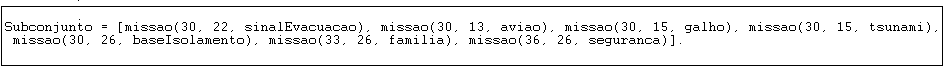
\includegraphics[keepaspectratio=true,scale=0.7]{figuras/resultado1.png}
\caption{Retorno do Cenário de Teste 1 aplicado no \textit{algoritmoDeDecisao}}
\label{resultado1}
\end{figure}
 

Quanto aos pontos X e Y das missões, a Tabela \ref{pontoCT1} mostra quais os pontos finais das missões dos subconjunto ótimo, lembrando que o ponto inicial é x = 0 e y = 0. A Figura \ref{stringCT1} mostra o retorno do componente \textit{stringDePontos} criado a partir componente \textit{escritaPontosEmArquivo}, que recebeu como entrada o subconjunto ótimo do Cenário de Teste 1. 

Comparando os pontos finais da Tabela e da Figura, é possível perceber que o componente gerou a saída corretamente.


\begin{table}[!h]
\centering
\caption{Pontos das Missões do Subconjunto Ótimo do Cenário de Teste 1}
\label{pontoCT1}
\begin{tabular}{lcc}
\rowcolor[HTML]{00D2CB} 
\multicolumn{1}{c}{\cellcolor[HTML]{00D2CB}} & \multicolumn{2}{l}{\cellcolor[HTML]{00D2CB}Ponto Final} \\ 
\rowcolor[HTML]{C0F2F0} 
\multicolumn{1}{c}{\cellcolor[HTML]{00D2CB}Missão} & \multicolumn{1}{c}{\cellcolor[HTML]{C0F2F0}X} & \multicolumn{1}{c}{\cellcolor[HTML]{C0F2F0}Y} \\
 Sinal de Evacuação & 65 & 18 \\
 Avião & 31 & 2 \\
 Galho & 14 & 33 \\
 Tsunami & 29 & 14 \\
 Base de Isolamento & 53 & 30 \\
 Família & 75 & 12 \\
 Segurança & 75 & 12    \\          
\end{tabular}
\end{table}


\FloatBarrier
\begin{figure}[!h]
\centering
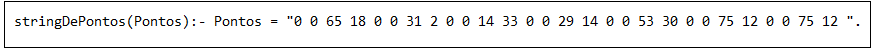
\includegraphics[keepaspectratio=true,scale=0.7]{figuras/stringCT1.png}
\caption{\textit{String} De Pontos gerada para o Cenário de Teste 1}
\label{stringCT1}
\end{figure}



\section{Cenário de teste 2}

	O segundo Cenário de Teste também obteve sucesso, pois o resultado gerado pela Tabela \ref{gabarito2} é idêntico ao gerado pelo componente \textit{algoritmoDeDecisão} mostrado na Figura \ref{resultado2}.
	
\begin{table}[!h]
\centering
\caption{Gabarito do Cenário de Teste 2}
\label{gabarito2}
\begin{tabular}{lccccccccccc}
\multicolumn{1}{c}{\cellcolor[HTML]{00D2CB}} & \multicolumn{11}{c}{\cellcolor[HTML]{00D2CB}\textbf{Tempo Restante}} \\ \multicolumn{1}{c}{\cellcolor[HTML]{00D2CB}{\color[HTML]{333333} \textbf{\{Valor\} Missão(Tempo)}}} & 
\multicolumn{1}{l}{\cellcolor[HTML]{C0F2F0}\textbf{0}} & 
\multicolumn{1}{l}{\cellcolor[HTML]{C0F2F0}\textbf{15}} & 
\multicolumn{1}{l}{\cellcolor[HTML]{C0F2F0}\textbf{30}} & 
\multicolumn{1}{l}{\cellcolor[HTML]{C0F2F0}\textbf{45}} & 
\multicolumn{1}{l}{\cellcolor[HTML]{C0F2F0}\textbf{60}} & 
\multicolumn{1}{l}{\cellcolor[HTML]{C0F2F0}\textbf{75}} & 
\multicolumn{1}{l}{\cellcolor[HTML]{C0F2F0}\textbf{90}} & 
\multicolumn{1}{l}{\cellcolor[HTML]{C0F2F0}\textbf{105}} & 
\multicolumn{1}{l}{\cellcolor[HTML]{C0F2F0}\textbf{120}} & 
\multicolumn{1}{l}{\cellcolor[HTML]{C0F2F0}\textbf{135}} & 
\multicolumn{1}{l}{\cellcolor[HTML]{C0F2F0}\textbf{150}} \\ 
0 & 0 & 0 & 0 & 0 & 0 & 0 & 0 & 0 & 0 & 0 & 0  \\ 
\{30\}  Avião(13) & 0 & 30 & 30 & 30 & 30 & 30 & 30 & 30 & 30 & 30 & 30 \\ 
\{30\}  Galho(15) & 0 & 30 & 60 & 60 & 60 & 60 & 60 & 60 & 60 & 60 & 60  \\ 
\{30\}  Tsunami(15) & 0 & 30 & 60 & 90 & 90 & 90 & 90 & 90 & 90 & 90 & 90 \\ 
\{30\}  Sinal de Evacuação (22) & 0 & 30 & 60 & 90 & 90 & 120  & 120  & 120 & 120 & 120 & 120 \\
\{20\}  Caminhão (28) & 0 & 30 & 60 & 90 & 90  & 120  & 120  & 140 & 140 & 140 & 140 \\ 
\{25\}  Ambulância (30) & 0 & 30 & 60 & 90 & 90  & 120  & 120  & 145 & 145 & 165 & 165 \\ 
{\color[HTML]{FE0000} \{20\}  Realocação (37)} & 0 & 30 & 60 & 90 & 90  & 120  & 120  & 145 & 145 & 165 & 165 \\  
\end{tabular}
\end{table}


\FloatBarrier
\begin{figure}[!h]
\centering
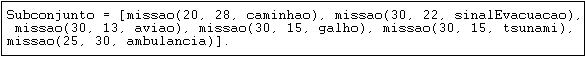
\includegraphics[keepaspectratio=true,scale=0.7]{figuras/resultado2.png}
\caption{Retorno do Cenário de Teste 2 aplicado no \textit{algoritmoDeDecisao}}
\label{resultado2}
\end{figure}

	Os pontos X e Y da Tabela \ref{pontoCT2} conferem com os pontos da saída gerada pelo componente \textit{stringDePontos} mostrado na Figura \ref{stringCT2}.

\begin{table}[!h]
\centering
\caption{Pontos das Missões do Subconjunto Ótimo do Cenário de Teste 2}
\label{pontoCT2}
\begin{tabular}{lcc}
\rowcolor[HTML]{00D2CB} 
\multicolumn{1}{c}{\cellcolor[HTML]{00D2CB}} & \multicolumn{2}{l}{\cellcolor[HTML]{00D2CB}Ponto Final} \\ 
\rowcolor[HTML]{C0F2F0} 
\multicolumn{1}{c}{\cellcolor[HTML]{00D2CB}Missão} & \multicolumn{1}{c}{\cellcolor[HTML]{C0F2F0}X} & \multicolumn{1}{c}{\cellcolor[HTML]{C0F2F0}Y} \\
 Caminhão & 12 & 21 \\
 Sinal de Evacuação & 65 & 18 \\
 Avião & 31 & 2 \\
 Galho & 14 & 33 \\
 Tsunami & 29 & 14 \\
 Ambulância & 33 & 22 \\          
\end{tabular}
\end{table}


\FloatBarrier
\begin{figure}[!h]
\centering
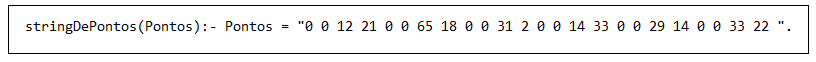
\includegraphics[keepaspectratio=true,scale=0.7]{figuras/stringCT2.png}
\caption{\textit{String} De Pontos gerada para o Cenário de Teste 2}
\label{stringCT2}
\end{figure}



\section{Cenário de teste 3}

	O terceiro Cenário de Teste obteve sucesso, assim como os seus anteriores. A Tabela \ref{gabarito3} confere com a saída mostrada na Figura \ref{resultado3}.
	
\begin{table}[!h]
\centering
\caption{Gabarito do Cenário de Teste 3}
\label{gabarito3}
\begin{tabular}{lccccccccccc}
\multicolumn{1}{c}{\cellcolor[HTML]{00D2CB}} & \multicolumn{11}{c}{\cellcolor[HTML]{00D2CB}\textbf{Tempo Restante}} \\ 
\multicolumn{1}{c}{\cellcolor[HTML]{00D2CB}{\color[HTML]{333333} \textbf{\{Valor\} Missão(Tempo)}}} & 
\multicolumn{1}{l}{\cellcolor[HTML]{C0F2F0}\textbf{0}} & 
\multicolumn{1}{l}{\cellcolor[HTML]{C0F2F0}\textbf{15}} & 
\multicolumn{1}{l}{\cellcolor[HTML]{C0F2F0}\textbf{30}} & 
\multicolumn{1}{l}{\cellcolor[HTML]{C0F2F0}\textbf{45}} & 
\multicolumn{1}{l}{\cellcolor[HTML]{C0F2F0}\textbf{60}} & 
\multicolumn{1}{l}{\cellcolor[HTML]{C0F2F0}\textbf{75}} & 
\multicolumn{1}{l}{\cellcolor[HTML]{C0F2F0}\textbf{90}} & 
\multicolumn{1}{l}{\cellcolor[HTML]{C0F2F0}\textbf{105}} & 
\multicolumn{1}{l}{\cellcolor[HTML]{C0F2F0}\textbf{120}} & 
\multicolumn{1}{l}{\cellcolor[HTML]{C0F2F0}\textbf{135}} & 
\multicolumn{1}{l}{\cellcolor[HTML]{C0F2F0}\textbf{150}} \\ 
0 & 0 & 0 & 0 & 0 & 0 & 0 & 0 & 0 & 0 & 0 & 0  \\ 
\{25\}  Elevar a Casa(15)& 0 & 25 & 25 & 25 & 25  & 25  & 25  & 25 & 25 & 25 & 25 \\ 
\{30\}  Base de Isolamento (26) & 0 & 25 & 30 & 55 & 55  & 55  & 55  & 55 & 55 & 55 & 55 \\ 
\{33\}  Família (26) & 0 & 25 & 33 & 58 & 63  & 88  & 88  & 88 & 88 & 88 & 88 \\ 
\{26\}  Segurança (26) & 0 & 25 & 36 & 61 & 69  & 94  & 99  & 124 & 124 & 124 & 124 \\ 
{\color[HTML]{FE0000} \{20\}  Realocação (37)} & 0 & 25 & 36 & 61 & 69  & 94  & 99  & 124 & 124 & 144 & 144 \\ 
\{31\}  Obstáculos (40) & 0 & 25 & 36 & 61 & 69  & 94  & 99  & 124 & 130 & 155 & 155 \\ 
\end{tabular}
\end{table}

	
\FloatBarrier
\begin{figure}[!h]
\centering
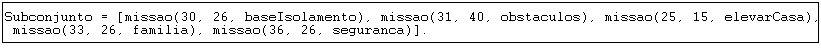
\includegraphics[keepaspectratio=true,scale=0.7]{figuras/resultado3.png}
\caption{Retorno do Cenário de Teste 3 aplicado no \textit{algoritmoDeDecisao}}
\label{resultado3}
\end{figure}


	Os pontos X e Y mostrados na Tabela \ref{pontoCT3} e na Figura \ref{stringCT3} também conferem.
	
\begin{table}[!h]
\centering
\caption{Pontos das Missões do Subconjunto Ótimo do Cenário de Teste 3}
\label{pontoCT3}
\begin{tabular}{lcc}
\rowcolor[HTML]{00D2CB} 
\multicolumn{1}{c}{\cellcolor[HTML]{00D2CB}} & \multicolumn{2}{l}{\cellcolor[HTML]{00D2CB}Ponto Final} \\ 
\rowcolor[HTML]{C0F2F0} 
\multicolumn{1}{c}{\cellcolor[HTML]{00D2CB}Missão} & \multicolumn{1}{c}{\cellcolor[HTML]{C0F2F0}X} & \multicolumn{1}{c}{\cellcolor[HTML]{C0F2F0}Y} \\
 Base de Isolamento & 53 & 30 \\
 Obstáculos & 75 & 8 \\
 Elevar a Casa & 34 & 26 \\
 Família & 75 & 12 \\
 Segurança & 75 & 12    \\          
\end{tabular}
\end{table}


\FloatBarrier
\begin{figure}[!h]
\centering
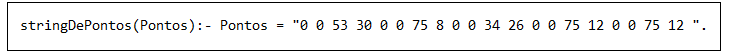
\includegraphics[keepaspectratio=true,scale=0.7]{figuras/stringCT3.png}
\caption{\textit{String} De Pontos gerada para o Cenário de Teste 3}
\label{stringCT3}
\end{figure}



\section{Cenário de teste 4}

	O quarto Cenário de Teste, não diferente dos demais, obteve sucesso tanto no subconjunto ótimo, mostrado pela Tabela \ref{gabarito4} e a Figura \ref{resultado4}, quanto nos pontos, mostrados na Tabela \ref{pontoCT4} e na Figura \ref{stringCT4}.

\begin{table}[!h]
\centering
\caption{Gabarito do Cenário de Teste 4}
\label{gabarito4}
\begin{tabular}{lccccccccccc}
\multicolumn{1}{c}{\cellcolor[HTML]{00D2CB}} & \multicolumn{11}{c}{\cellcolor[HTML]{00D2CB}\textbf{Tempo Restante}} \\ 
\multicolumn{1}{c}{\cellcolor[HTML]{00D2CB}{\color[HTML]{333333} \textbf{\{Valor\} Missão(Tempo)}}} & 
\multicolumn{1}{l}{\cellcolor[HTML]{C0F2F0}\textbf{0}} & 
\multicolumn{1}{l}{\cellcolor[HTML]{C0F2F0}\textbf{15}} & 
\multicolumn{1}{l}{\cellcolor[HTML]{C0F2F0}\textbf{30}} & 
\multicolumn{1}{l}{\cellcolor[HTML]{C0F2F0}\textbf{45}} & 
\multicolumn{1}{l}{\cellcolor[HTML]{C0F2F0}\textbf{60}} & 
\multicolumn{1}{l}{\cellcolor[HTML]{C0F2F0}\textbf{75}} & 
\multicolumn{1}{l}{\cellcolor[HTML]{C0F2F0}\textbf{90}} & 
\multicolumn{1}{l}{\cellcolor[HTML]{C0F2F0}\textbf{105}} & 
\multicolumn{1}{l}{\cellcolor[HTML]{C0F2F0}\textbf{120}} & 
\multicolumn{1}{l}{\cellcolor[HTML]{C0F2F0}\textbf{135}} & 
\multicolumn{1}{l}{\cellcolor[HTML]{C0F2F0}\textbf{150}} \\ 
0 & 0 & 0 & 0 & 0 & 0 & 0 & 0 & 0 & 0 & 0 & 0  \\ 
\{30\}  Avião(13) & 0 & 30 & 30 & 30 & 30 & 30 & 30 & 30 & 30 & 30 & 30 \\ 
\{30\}  Galho(15) & 0 & 30 & 60 & 60 & 60 & 60 & 60 & 60 & 60 & 60 & 60  \\ 
\{30\}  Tsunami(15) & 0 & 30 & 60 & 90 & 90 & 90 & 90 & 90 & 90 & 90 & 90 \\ 
\{30\}  Base de Isolamento (26) & 0 & 30 & 60 & 90 & 90 & 120  & 120  & 120 & 120 & 120 & 120 \\ 
\{33\}  Família (26) & 0 & 30 & 60 & 90 & 93  & 123  & 153  & 153 & 153 & 153 & 153 \\ 
\{25\}  Ambulância (30) & 0 & 30 & 60 & 90 & 93  & 123  & 153  & 153 & 153 & 178 & 178 \\ 
{\color[HTML]{FE0000} \{20\}  Realocação (37)} & 0 & 30 & 60 & 90 & 93  & 123  & 153  & 153 & 153 & 178 & 178 \\ 
\end{tabular}
\end{table}


\FloatBarrier
\begin{figure}[!h]
\centering
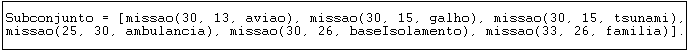
\includegraphics[keepaspectratio=true,scale=0.7]{figuras/resultado4.png}
\caption{Retorno do Cenário de Teste 4 aplicado no \textit{algoritmoDeDecisao}}
\label{resultado4}
\end{figure}


\begin{table}[!h]
\centering
\caption{Pontos das Missões do Subconjunto Ótimo do Cenário de Teste 4}
\label{pontoCT4}
\begin{tabular}{lcc}
\rowcolor[HTML]{00D2CB} 
\multicolumn{1}{c}{\cellcolor[HTML]{00D2CB}} & \multicolumn{2}{l}{\cellcolor[HTML]{00D2CB}Ponto Final} \\ 
\rowcolor[HTML]{C0F2F0} 
\multicolumn{1}{c}{\cellcolor[HTML]{00D2CB}Missão} & \multicolumn{1}{c}{\cellcolor[HTML]{C0F2F0}X} & \multicolumn{1}{c}{\cellcolor[HTML]{C0F2F0}Y} \\
 Avião & 31 & 2 \\
 Galho & 14 & 33 \\
 Tsunami & 29 & 14 \\
 Ambulância & 33 & 22 \\
 Base de Isolamento & 53 & 30 \\
 Família & 75 & 12 \\          
\end{tabular}
\end{table}


\FloatBarrier
\begin{figure}[!h]
\centering
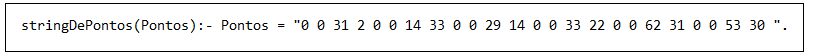
\includegraphics[keepaspectratio=true,scale=0.7]{figuras/stringCT4.png}
\caption{\textit{String} De Pontos gerada para o Cenário de Teste 4}
\label{stringCT4}
\end{figure}



\section{Cenário de teste 5}

	O quinto Cenário de Teste, conforme a Tabela \ref{gabarito5} e a Figura \ref{resultado5}, também obteve sucesso ao gerar o subconjunto ótimo. Quanto aos pontos iniciais e finais, a Tabela \ref{pontoCT5} e a Figura \ref{stringCT5} demostram que o cenário obteve sucesso.
	
\begin{table}[!h]
\centering
\caption{Gabarito do Cenário de Teste 5}
\label{gabarito5}
\begin{tabular}{lccccccccccc}
\multicolumn{1}{c}{\cellcolor[HTML]{00D2CB}} & \multicolumn{11}{c}{\cellcolor[HTML]{00D2CB}\textbf{Tempo Restante}} \\ 
\multicolumn{1}{c}{\cellcolor[HTML]{00D2CB}{\color[HTML]{333333} \textbf{\{Valor\} Missão(Tempo)}}} & 
\multicolumn{1}{l}{\cellcolor[HTML]{C0F2F0}\textbf{0}} & 
\multicolumn{1}{l}{\cellcolor[HTML]{C0F2F0}\textbf{15}} & 
\multicolumn{1}{l}{\cellcolor[HTML]{C0F2F0}\textbf{30}} & 
\multicolumn{1}{l}{\cellcolor[HTML]{C0F2F0}\textbf{45}} & 
\multicolumn{1}{l}{\cellcolor[HTML]{C0F2F0}\textbf{60}} & 
\multicolumn{1}{l}{\cellcolor[HTML]{C0F2F0}\textbf{75}} & 
\multicolumn{1}{l}{\cellcolor[HTML]{C0F2F0}\textbf{90}} & 
\multicolumn{1}{l}{\cellcolor[HTML]{C0F2F0}\textbf{105}} & 
\multicolumn{1}{l}{\cellcolor[HTML]{C0F2F0}\textbf{120}} & 
\multicolumn{1}{l}{\cellcolor[HTML]{C0F2F0}\textbf{135}} & 
\multicolumn{1}{l}{\cellcolor[HTML]{C0F2F0}\textbf{150}} \\ 
0 & 0 & 0 & 0 & 0 & 0 & 0 & 0 & 0 & 0 & 0 & 0  \\ 
\{30\}  Avião(13) & 0 & 30 & 30 & 30 & 30 & 30 & 30 & 30 & 30 & 30 & 30 \\ 
\{30\}  Tsunami(15) & 0 & 30 & 60 & 60 & 60 & 60 & 60 & 60 & 60 & 60 & 60 \\ 
{\color[HTML]{FE0000} \{25\}  Elevar a Casa(15)}& 0 & 30 & 60 & 85 & 85  & 85  & 85  & 85 & 85 & 85 & 85 \\ 
\{30\}  Base de Isolamento (26) & 0 & 30 & 60 & 85 & 90  & 115  & 115  & 115 & 115 & 115 & 115 \\ 
\{33\}  Família (26) & 0 & 30 & 60 & 85 & 93  & 118 & 123  & 148 & 148 & 148 & 148 \\ 
\{26\}  Segurança (26) & 0 & 30 & 60 & 85 & 96 & 121  & 129  & 154 & 159 & 184 & 184 \\ 
{\color[HTML]{FE0000} \{20\}  Realocação (37)} & 0 & 30 & 60 & 85 & 96 & 121  & 129  & 154 & 159 & 184 & 184 \\ 
\{31\}  Obstáculos (40) & 0 & 30 & 60 & 85 & 96 & 121  & 129  & 154 & 160 & 185 & 190 \\ 
\end{tabular}
\end{table}


\FloatBarrier
\begin{figure}[!h]
\centering
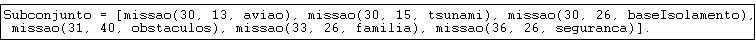
\includegraphics[keepaspectratio=true,scale=0.7]{figuras/resultado5.png}
\caption{Retorno do Cenário de Teste 5 aplicado no \textit{algoritmoDeDecisao}}
\label{resultado5}
\end{figure}


\begin{table}[!h]
\centering
\caption{Pontos das Missões do Subconjunto Ótimo do Cenário de Teste 5}
\label{pontoCT5}
\begin{tabular}{lcc}
\rowcolor[HTML]{00D2CB} 
\multicolumn{1}{c}{\cellcolor[HTML]{00D2CB}} & \multicolumn{2}{l}{\cellcolor[HTML]{00D2CB}Ponto Final} \\ 
\rowcolor[HTML]{C0F2F0} 
\multicolumn{1}{c}{\cellcolor[HTML]{00D2CB}Missão} & \multicolumn{1}{c}{\cellcolor[HTML]{C0F2F0}X} & \multicolumn{1}{c}{\cellcolor[HTML]{C0F2F0}Y} \\
 Avião & 31 & 2 \\
 Tsunami & 29 & 14 \\
 Base de Isolamento & 53 & 30 \\
 Obstáculos & 75 & 8 \\
 Família & 75 & 12 \\
 Segurança & 75 & 12    \\          
\end{tabular}
\end{table}


\FloatBarrier
\begin{figure}[!h]
\centering
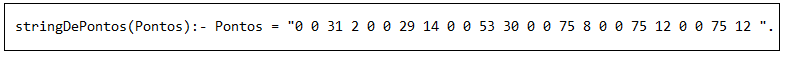
\includegraphics[keepaspectratio=true,scale=0.7]{figuras/stringCT5.png}
\caption{\textit{String} De Pontos gerada para o Cenário de Teste 5}
\label{stringCT5}
\end{figure}



\section{Cenário de teste 6}

	O sexto Cenário de Teste obteve sucesso nos dois pontos analisados: tanto na geração do subconjunto ótimo quanto na geração da \textit{string} de pontos. A Tabela \ref{gabarito6} e a Figura \ref{resultado6} demonstram o sucesso no primeiro ponto analisado, enquanto a Tabela \ref{pontoCT6} e a Figura \ref{stringCT6} demonstram o sucesso do segundo ponto.

\begin{table}[!h]
\centering
\caption{Gabarito do Cenário de Teste 6}
\label{gabarito6}
\begin{tabular}{lccccccccccc}
\multicolumn{1}{c}{\cellcolor[HTML]{00D2CB}} & \multicolumn{11}{c}{\cellcolor[HTML]{00D2CB}\textbf{Tempo Restante}} \\ 
\multicolumn{1}{c}{\cellcolor[HTML]{00D2CB}{\color[HTML]{333333} \textbf{\{Valor\} Missão(Tempo)}}} & 
\multicolumn{1}{l}{\cellcolor[HTML]{C0F2F0}\textbf{0}} & 
\multicolumn{1}{l}{\cellcolor[HTML]{C0F2F0}\textbf{15}} & 
\multicolumn{1}{l}{\cellcolor[HTML]{C0F2F0}\textbf{30}} & 
\multicolumn{1}{l}{\cellcolor[HTML]{C0F2F0}\textbf{45}} & 
\multicolumn{1}{l}{\cellcolor[HTML]{C0F2F0}\textbf{60}} & 
\multicolumn{1}{l}{\cellcolor[HTML]{C0F2F0}\textbf{75}} & 
\multicolumn{1}{l}{\cellcolor[HTML]{C0F2F0}\textbf{90}} & 
\multicolumn{1}{l}{\cellcolor[HTML]{C0F2F0}\textbf{105}} & 
\multicolumn{1}{l}{\cellcolor[HTML]{C0F2F0}\textbf{120}} & 
\multicolumn{1}{l}{\cellcolor[HTML]{C0F2F0}\textbf{135}} & 
\multicolumn{1}{l}{\cellcolor[HTML]{C0F2F0}\textbf{150}} \\ 
0 & 0 & 0 & 0 & 0 & 0 & 0 & 0 & 0 & 0 & 0 & 0  \\ 
\{30\}  Avião(13) & 0 & 30 & 30 & 30 & 30 & 30 & 30 & 30 & 30 & 30 & 30 \\ 
\{30\}  Galho(15) & 0 & 30 & 60 & 60 & 60 & 60 & 60 & 60 & 60 & 60 & 60  \\ 
\{25\}  Elevar a Casa(15)& 0 & 30 & 60 & 85 & 85  & 85  & 85  & 85 & 85 & 85 & 85 \\ 
\{30\}  Sinal de Evacuação (22) & 0 & 30 & 60 & 85 & 90 & 115 & 115  & 115 & 115 & 115 & 115 \\ 
\{33\}  Família (26) & 0 & 30 & 60 & 85 & 93  & 118  & 123  & 148 & 148 & 148 & 148 \\ 
\{26\}  Segurança (26) & 0 & 30 & 60 & 85 & 96  & 121  & 129  & 154 & 184 & 184 & 184 \\ 
\{20\}  Caminhão (28) & 0 & 30 & 60 & 85 & 96  & 121  & 129  & 154 & 184 & 184 & 204 \\ 
{\color[HTML]{FE0000} \{31\}  Obstáculos (40)} & 0 & 30 & 60 & 85 & 96  & 121  & 129  & 154 & 184 & 185 & 184 \\ 
\end{tabular}
\end{table}


\FloatBarrier
\begin{figure}[!h]
\centering
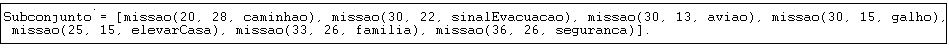
\includegraphics[keepaspectratio=true,scale=0.7]{figuras/resultado6.png}
\caption{Retorno do Cenário de Teste 6 aplicado no \textit{algoritmoDeDecisao}}
\label{resultado6}
\end{figure}


\begin{table}[!h]
\centering
\caption{Pontos das Missões do Subconjunto Ótimo do Cenário de Teste 6}
\label{pontoCT6}
\begin{tabular}{lcc}
\rowcolor[HTML]{00D2CB} 
\multicolumn{1}{c}{\cellcolor[HTML]{00D2CB}} & \multicolumn{2}{l}{\cellcolor[HTML]{00D2CB}Ponto Final} \\ 
\rowcolor[HTML]{C0F2F0} 
\multicolumn{1}{c}{\cellcolor[HTML]{00D2CB}Missão} & \multicolumn{1}{c}{\cellcolor[HTML]{C0F2F0}X} & \multicolumn{1}{c}{\cellcolor[HTML]{C0F2F0}Y} \\
 Caminhão & 12 & 21 \\
 Sinal de Evacuação & 65 & 18 \\
 Avião & 31 & 2 \\
 Galho & 14 & 33 \\
 Elevar a Casa & 34 & 26 \\
 Família & 75 & 12 \\
 Segurança & 75 & 12    \\          
\end{tabular}
\end{table}


\FloatBarrier
\begin{figure}[!h]
\centering
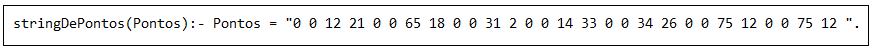
\includegraphics[keepaspectratio=true,scale=0.7]{figuras/stringCT6.png}
\caption{\textit{String} De Pontos gerada para o Cenário de Teste 6}
\label{stringCT6}
\end{figure}



\section{Cenário de teste 7}

	O sétimo Cenário de Uso obteve sucesso na geração do subconjunto ótimo, como demostra a Tabela \ref{gabarito7} e a Figura \ref{resultado7}. Obteve sucesso também na geração da \textit{string} de pontos, conforme Tabela \ref{pontoCT7} e Figura \ref{stringCT7}.

\begin{table}[!h]
\centering
\caption{Gabarito do Cenário de Teste 7}
\label{gabarito7}
\begin{tabular}{lccccccccccc}
\multicolumn{1}{c}{\cellcolor[HTML]{00D2CB}} & \multicolumn{11}{c}{\cellcolor[HTML]{00D2CB}\textbf{Tempo Restante}} \\ 
\multicolumn{1}{c}{\cellcolor[HTML]{00D2CB}{\color[HTML]{333333} \textbf{\{Valor\} Missão(Tempo)}}} & 
\multicolumn{1}{l}{\cellcolor[HTML]{C0F2F0}\textbf{0}} & 
\multicolumn{1}{l}{\cellcolor[HTML]{C0F2F0}\textbf{15}} & 
\multicolumn{1}{l}{\cellcolor[HTML]{C0F2F0}\textbf{30}} & 
\multicolumn{1}{l}{\cellcolor[HTML]{C0F2F0}\textbf{45}} & 
\multicolumn{1}{l}{\cellcolor[HTML]{C0F2F0}\textbf{60}} & 
\multicolumn{1}{l}{\cellcolor[HTML]{C0F2F0}\textbf{75}} & 
\multicolumn{1}{l}{\cellcolor[HTML]{C0F2F0}\textbf{90}} & 
\multicolumn{1}{l}{\cellcolor[HTML]{C0F2F0}\textbf{105}} & 
\multicolumn{1}{l}{\cellcolor[HTML]{C0F2F0}\textbf{120}} & 
\multicolumn{1}{l}{\cellcolor[HTML]{C0F2F0}\textbf{135}} & 
\multicolumn{1}{l}{\cellcolor[HTML]{C0F2F0}\textbf{150}} \\ 
0 & 0 & 0 & 0 & 0 & 0 & 0 & 0 & 0 & 0 & 0 & 0  \\ 
\{30\}  Tsunami(15) & 0 & 30 & 30 & 30 & 30 & 30 & 30 & 30 & 30 & 30 & 30 \\ 
\{30\}  Base de Isolamento (26) & 0 & 30 & 30 & 60 & 60  & 60  & 60  & 60 & 60 & 60 & 60 \\ 
\{33\}  Família (26) & 0 & 30 & 33 & 63 & 63  & 93  & 93 & 93 & 93 & 93 & 93 \\ 
\{26\}  Segurança (26) & 0 & 30 & 36 & 66 & 69  & 99  & 99 & 129 & 129 & 129 & 129 \\ 
\{25\}  Ambulância (30) & 0 & 30 & 36 & 66 & 69  & 99  & 99 & 129 & 129 & 154 & 154 \\ 
{\color[HTML]{FE0000} \{20\}  Realocação (37)} & 0 & 30 & 36 & 66 & 69  & 99  & 99 & 129 & 129 & 154 & 154 \\  
\end{tabular}
\end{table}


\FloatBarrier
\begin{figure}[!h]
\centering
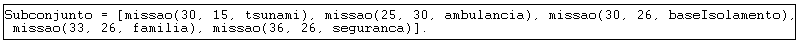
\includegraphics[keepaspectratio=true,scale=0.7]{figuras/resultado7.png}
\caption{Retorno do Cenário de Teste 7 aplicado no \textit{algoritmoDeDecisao}}
\label{resultado7}
\end{figure}


\begin{table}[!h]
\centering
\caption{Pontos das Missões do Subconjun|to Ótimo do Cenário de Teste 7}
\label{pontoCT7}
\begin{tabular}{lcc}
\rowcolor[HTML]{00D2CB} 
\multicolumn{1}{c}{\cellcolor[HTML]{00D2CB}} & \multicolumn{2}{l}{\cellcolor[HTML]{00D2CB}Ponto Final} \\ 
\rowcolor[HTML]{C0F2F0} 
\multicolumn{1}{c}{\cellcolor[HTML]{00D2CB}Missão} & \multicolumn{1}{c}{\cellcolor[HTML]{C0F2F0}X} & \multicolumn{1}{c}{\cellcolor[HTML]{C0F2F0}Y} \\
 Tsunami & 29 & 14 \\
 Ambulância & 33 & 22 \\
 Base de Isolamento & 53 & 30 \\
 Família & 75 & 12 \\
 Segurança & 75 & 12    \\          
\end{tabular}
\end{table}


\FloatBarrier
\begin{figure}[!h]
\centering
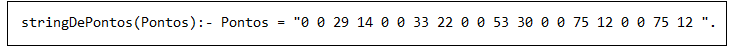
\includegraphics[keepaspectratio=true,scale=0.7]{figuras/stringCT7.png}
\caption{\textit{String} De Pontos gerada para o Cenário de Teste 7}
\label{stringCT7}
\end{figure}



\section{Cenário de teste 8}

	Segundo a Tabela \ref{gabarito8} e a Figura \ref{resultado8}, o quinto Cenário de Teste obteve sucesso no quesito geração do subconjunto ótimo. 

\begin{table}[!h]
\centering
\caption{Gabarito do Cenário de Teste 8}
\label{gabarito8}
\begin{tabular}{lccccccccccc}
\multicolumn{1}{c}{\cellcolor[HTML]{00D2CB}} & \multicolumn{11}{c}{\cellcolor[HTML]{00D2CB}\textbf{Tempo Restante}} \\ 
\multicolumn{1}{c}{\cellcolor[HTML]{00D2CB}{\color[HTML]{333333} \textbf{\{Valor\} Missão(Tempo)}}} & 
\multicolumn{1}{l}{\cellcolor[HTML]{C0F2F0}\textbf{0}} & 
\multicolumn{1}{l}{\cellcolor[HTML]{C0F2F0}\textbf{15}} & 
\multicolumn{1}{l}{\cellcolor[HTML]{C0F2F0}\textbf{30}} & 
\multicolumn{1}{l}{\cellcolor[HTML]{C0F2F0}\textbf{45}} & 
\multicolumn{1}{l}{\cellcolor[HTML]{C0F2F0}\textbf{60}} & 
\multicolumn{1}{l}{\cellcolor[HTML]{C0F2F0}\textbf{75}} & 
\multicolumn{1}{l}{\cellcolor[HTML]{C0F2F0}\textbf{90}} & 
\multicolumn{1}{l}{\cellcolor[HTML]{C0F2F0}\textbf{105}} & 
\multicolumn{1}{l}{\cellcolor[HTML]{C0F2F0}\textbf{120}} & 
\multicolumn{1}{l}{\cellcolor[HTML]{C0F2F0}\textbf{135}} & 
\multicolumn{1}{l}{\cellcolor[HTML]{C0F2F0}\textbf{150}} \\ 
0 & 0 & 0 & 0 & 0 & 0 & 0 & 0 & 0 & 0 & 0 & 0  \\ 
\{30\}  Tsunami(15) & 0 & 30 & 30 & 30 & 30 & 30 & 30 & 30 & 30 & 30 & 30 \\  
\{30\}  Sinal de Evacuação (22) &  0 & 30 & 30 & 60 & 60 & 60 & 60 & 60 & 60 & 60 & 60 \\ 
\{33\}  Família (26) & 0 & 30 & 33 & 63 & 63 & 93 & 93 & 93 & 93 & 93 & 93  \\ 
\{26\}  Segurança (26) & 0 & 30 & 36 & 66 & 66 & 96 & 129 & 129 & 129 & 129 & 129 \\ 
\{25\}  Ambulância (30) & 0 & 30 & 36 & 66 & 66 & 96 & 129 & 129 & 154 & 154 & 154 \\ 
{\color[HTML]{FE0000} \{20\}  Realocação (37)} & 0 & 30 & 36 & 66 & 66 & 96 & 129 & 129 & 154 & 154 & 154 \\ 
\end{tabular}
\end{table}


\FloatBarrier
\begin{figure}[!h]
\centering
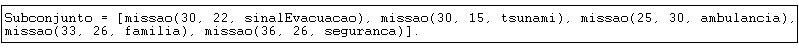
\includegraphics[keepaspectratio=true,scale=0.7]{figuras/resultado8.png}
\caption{Retorno do Cenário de Teste 8 aplicado no \textit{algoritmoDeDecisao}}
\label{resultado8}
\end{figure}

	Conforme consta na Tabela \ref{pontoCT8} e na Figura \ref{stringCT8}, o oitavo Cenário de Teste também obteve sucesso no quesito geração da string de pontos.

\begin{table}[!h]
\centering
\caption{Pontos das Missões do Subconjunto Ótimo do Cenário de Teste 8}
\label{pontoCT8}
\begin{tabular}{lcc}
\rowcolor[HTML]{00D2CB} 
\multicolumn{1}{c}{\cellcolor[HTML]{00D2CB}} & \multicolumn{2}{l}{\cellcolor[HTML]{00D2CB}Ponto Final} \\ 
\rowcolor[HTML]{C0F2F0} 
\multicolumn{1}{c}{\cellcolor[HTML]{00D2CB}Missão} & \multicolumn{1}{c}{\cellcolor[HTML]{C0F2F0}X} & \multicolumn{1}{c}{\cellcolor[HTML]{C0F2F0}Y} \\
 Sinal de Evacuação & 65 & 18 \\
 Tsunami & 29 & 14 \\
 Ambulância & 33 & 22 \\
 Família & 75 & 12 \\
 Segurança & 75 & 12    \\          
\end{tabular}
\end{table}


\FloatBarrier
\begin{figure}[!h]
\centering
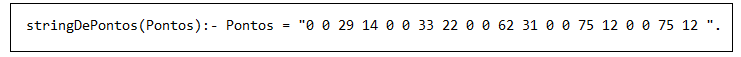
\includegraphics[keepaspectratio=true,scale=0.7]{figuras/stringCT8.png}
\caption{\textit{String} De Pontos gerada para o Cenário de Teste 8}
\label{stringCT8}
\end{figure}



\section{Cenário de teste 9}

	O último cenário de teste também obteve sucesso nos dois quesitos: geração do subconjunto ótimo de geração da \textit{string }de pontos. A Tabela \ref{gabarito9} e a Figura \ref{resultado9} comprovam o sucesso do nono Cenário de Teste no primeiro quesito. E, comprovando o sucesso no segundo quesito, estão os resultados apresentados na Tabela \ref{pontoCT9} e na Figura \ref{stringCT9}.

\begin{table}[!h]
\centering
\caption{Gabarito do Cenário de Teste 9}
\label{gabarito9}
\begin{tabular}{lccccccccccc}
\multicolumn{1}{c}{\cellcolor[HTML]{00D2CB}} & \multicolumn{11}{c}{\cellcolor[HTML]{00D2CB}\textbf{Tempo Restante}} \\ 
\multicolumn{1}{c}{\cellcolor[HTML]{00D2CB}{\color[HTML]{333333} \textbf{\{Valor\} Missão(Tempo)}}} & 
\multicolumn{1}{l}{\cellcolor[HTML]{C0F2F0}\textbf{0}} & 
\multicolumn{1}{l}{\cellcolor[HTML]{C0F2F0}\textbf{15}} & 
\multicolumn{1}{l}{\cellcolor[HTML]{C0F2F0}\textbf{30}} & 
\multicolumn{1}{l}{\cellcolor[HTML]{C0F2F0}\textbf{45}} & 
\multicolumn{1}{l}{\cellcolor[HTML]{C0F2F0}\textbf{60}} & 
\multicolumn{1}{l}{\cellcolor[HTML]{C0F2F0}\textbf{75}} & 
\multicolumn{1}{l}{\cellcolor[HTML]{C0F2F0}\textbf{90}} & 
\multicolumn{1}{l}{\cellcolor[HTML]{C0F2F0}\textbf{105}} & 
\multicolumn{1}{l}{\cellcolor[HTML]{C0F2F0}\textbf{120}} & 
\multicolumn{1}{l}{\cellcolor[HTML]{C0F2F0}\textbf{135}} & 
\multicolumn{1}{l}{\cellcolor[HTML]{C0F2F0}\textbf{150}} \\ 
0 & 0 & 0 & 0 & 0 & 0 & 0 & 0 & 0 & 0 & 0 & 0  \\ 
\{30\}  Galho(15) & 0 & 30 & 30 & 30 & 30 & 30 & 30 & 30 & 30 & 30 & 30  \\ 
\{30\}  Tsunami(15) & 0 & 30 & 60 & 60 & 60 & 60 & 60 & 60 & 60 & 60 & 60 \\ 
\{25\}  Elevar a Casa(15)& 0 & 30 & 60 & 80 & 85  & 85  & 85  & 85 & 85 & 85 & 85 \\ 
\{30\}  Sinal de Evacuação (22) & 0 & 30 & 60 & 85 & 90  & 115  & 115  & 115 & 115 & 115 & 115 \\ 
\{30\}  Base de Isolamento (26) & 0 & 30 & 60 & 85 & 90  & 115  & 120  & 145 & 145 & 145 & 145 \\ 
\{33\}  Família (26) & 0 & 30 & 60 & 85 & 93  & 118  & 123  & 148 & 178 & 178 & 178 \\ 
\{26\}  Segurança (26) & 0 & 30 & 60 & 85 & 96  & 121  & 129  & 154 & 159 & 184 & 214 \\ 
{\color[HTML]{FE0000} \{20\}  Caminhão (28)} & 0 & 30 & 60 & 85 & 96  & 121  & 129  & 154 & 159 & 184 & 214 \\ 
{\color[HTML]{FE0000} \{25\}  Ambulância (30)} & 0 & 30 & 60 & 85 & 96  & 121  & 129  & 154 & 159 & 184 & 214 \\ 
{\color[HTML]{FE0000} \{20\}  Realocação (37)} & 0 & 30 & 60 & 85 & 96  & 121  & 129  & 154 & 159 & 184 & 214 \\ 
{\color[HTML]{FE0000} \{31\}  Obstáculos (40)} & 0 & 30 & 60 & 85 & 96  & 121  & 129  & 154 & 159 & 184 & 214 \\ 
\end{tabular}
\end{table}


\FloatBarrier
\begin{figure}[!h]
\centering
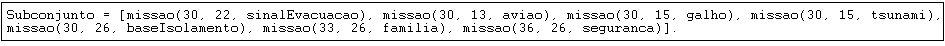
\includegraphics[keepaspectratio=true,scale=0.7]{figuras/resultado9.png}
\caption{Retorno do Cenário de Teste 9 aplicado no \textit{algoritmoDeDecisao}}
\label{resultado9}
\end{figure}


\begin{table}[!h]
\centering
\caption{Pontos das Missões do Subconjunto Ótimo do Cenário de Teste 9}
\label{pontoCT9}
\begin{tabular}{lcc}
\rowcolor[HTML]{00D2CB} 
\multicolumn{1}{c}{\cellcolor[HTML]{00D2CB}} & \multicolumn{2}{l}{\cellcolor[HTML]{00D2CB}Ponto Final} \\ 
\rowcolor[HTML]{C0F2F0} 
\multicolumn{1}{c}{\cellcolor[HTML]{00D2CB}Missão} & \multicolumn{1}{c}{\cellcolor[HTML]{C0F2F0}X} & \multicolumn{1}{c}{\cellcolor[HTML]{C0F2F0}Y} \\
 Sinal de Evacuação & 65 & 18 \\
 Avião & 31 & 2 \\
 Galho & 14 & 33 \\
 Tsunami & 29 & 14 \\
 Base de Isolamento & 53 & 30 \\
 Família & 75 & 12 \\
 Segurança & 75 & 12    \\          
\end{tabular}
\end{table}

\FloatBarrier
\begin{figure}[!h]
\centering
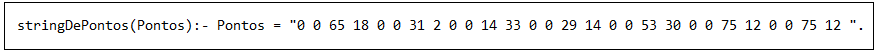
\includegraphics[keepaspectratio=true,scale=0.7]{figuras/stringCT9.png}
\caption{\textit{String} De Pontos gerada para o Cenário de Teste 9}
\label{stringCT9}
\end{figure}


\section{Considerações parciais}
	Os cenários de teste foram criados propositalmente com números variáveis de missões, para que fosse comprovada a eficiência da máquina com diversos tamanhos de entradas. Cada cenário de teste seguiu a regra de que o somatório dos tempos de execução das missões excedesse o tempo estipulado de 150 segundos, pois assim ao menos uma missão seria excluída pela máquina de raciocínio.
	Desta forma, todos os cenários de uso obtiveram sucesso nos quesitos analisados.